% =================================================================
% Trabajo Final Integrador — Tópicos en Aprendizaje Automático (UNAJ)
% Análisis crítico de "Patches Are All You Need?" (Trockman & Kolter)
% Compilar: pdflatex TF_informe.tex (dos pasadas). Los números salen de
% ../presentacion/resultados.tex, generado por src/figuras.py.
% =================================================================
\documentclass[11pt,a4paper]{article}
\usepackage{iftex}
\ifPDFTeX
  \usepackage[utf8]{inputenc}
  \usepackage[T1]{fontenc}
  \usepackage{lmodern}
\else
  \usepackage{fontspec}
\fi
\usepackage[spanish,es-noshorthands,es-nodecimaldot,es-tabla]{babel}
\usepackage[margin=2.3cm,headheight=38pt]{geometry}
\usepackage{graphicx,booktabs,array,tabularx,amsmath,amssymb,xcolor,enumitem,caption,fancyhdr,titlesec}
\usepackage[round]{natbib}
\usepackage[hidelinks]{hyperref}
\definecolor{unajazul}{HTML}{003366}
\titleformat{\section}{\large\bfseries\color{unajazul}}{\thesection.}{0.5em}{}
\titleformat{\subsection}{\normalsize\bfseries\color{unajazul}}{\thesubsection}{0.5em}{}
\graphicspath{{../presentacion/figuras/}}
% Generado por src/figuras.py a partir de results/*.json — no editar a mano
\providecommand{\accCMnueve}{82,7}
\providecommand{\paramsCMnueve}{223\,370}
\providecommand{\tputCMnueve}{422}
\providecommand{\minCMnueve}{110}
\providecommand{\valCMnueve}{83,1}
\providecommand{\entrCMnueve}{84,6}
\providecommand{\accCMtres}{84,6}
\providecommand{\paramsCMtres}{149\,642}
\providecommand{\tputCMtres}{531}
\providecommand{\minCMtres}{72}
\providecommand{\valCMtres}{85,4}
\providecommand{\entrCMtres}{86,2}
\providecommand{\accCMpcuatro}{78,7}
\providecommand{\paramsCMpcuatro}{227\,978}
\providecommand{\tputCMpcuatro}{1551}
\providecommand{\minCMpcuatro}{35}
\providecommand{\valCMpcuatro}{78,7}
\providecommand{\entrCMpcuatro}{78,8}
\providecommand{\accResNet}{83,0}
\providecommand{\paramsResNet}{308\,650}
\providecommand{\tputResNet}{1572}
\providecommand{\minResNet}{32}
\providecommand{\valResNet}{83,1}
\providecommand{\entrResNet}{83,7}
\providecommand{\epocasCNN}{10}
\providecommand{\accLineal}{40,7}
\providecommand{\lamCV}{10000}
\providecommand{\minLineal}{148}
\providecommand{\accPerceptron}{40,3}
\providecommand{\minPerceptron}{1}
\providecommand{\accMLP}{57,4}
\providecommand{\paramsMLP}{3\,676\,682}
\providecommand{\tputMLP}{14147}
\providecommand{\minMLP}{4}
\providecommand{\accELM}{47,3}
\providecommand{\LELM}{3000}
\providecommand{\paramsELM}{9\,249\,000}
\providecommand{\minELM}{3}
\providecommand{\accMLELM}{40,4}
\providecommand{\minMLELM}{9}
\providecommand{\ratioTput}{3,7}
\providecommand{\difCMResNet}{-0,3}
\providecommand{\difKernel}{-2,0}
\providecommand{\difKernelAbs}{2,0}
\providecommand{\difPatch}{4,0}
\providecommand{\accColab}{94,5}
\providecommand{\segColab}{56}
\providecommand{\epColab}{100}
\providecommand{\minColab}{93}
\providecommand{\minEpCPU}{11}
\providecommand{\colabNota}{al cabo de las 100 épocas}
\providecommand{\accKaggle}{95,48}
\providecommand{\segKaggle}{25}
\providecommand{\epKaggle}{200}
\providecommand{\minKaggle}{85}

\pagestyle{fancy}
\fancyhf{}
\fancyhead[L]{
\includegraphics[height=26pt]{logo_unaj.png}}
\fancyhead[R]{\small\bfseries Doctorado en Ciencia y Tecnología}
\fancyfoot[C]{\small\thepage}
\renewcommand{\headrulewidth}{0.4pt}
\setlength{\parskip}{0.45em}
\setlength{\parindent}{0pt}
\setlist{itemsep=0.15em,topsep=0.3em}
\newcommand{\pct}[1]{#1\,\%}
% Formato APA 7 para tablas y figuras: "Tabla 1" en negrita, título en cursiva en la línea siguiente, nota debajo
\captionsetup{labelfont=bf,textfont=it,labelsep=newline,justification=raggedright,singlelinecheck=false,skip=4pt}
\captionsetup[table]{name=Tabla}
\newcommand{\nota}[1]{\par\vspace{3pt}{\footnotesize\raggedright\textit{Nota.} #1\par}}

\begin{document}
\thispagestyle{fancy}
\begin{center}
  {\Large\bfseries Curso: Tópicos en Aprendizaje Automático}\\[0.4em]
  {\large Trabajo Final Integrador: Análisis Crítico de un Artículo Científico}\\[0.9em]
  {\Large\bfseries\color{unajazul} ¿Bastan los parches? Análisis y réplica parcial del ConvMixer}\\[0.5em]
  {\normalsize Trockman, A. y Kolter, J. Z. (2023). \emph{Patches Are All You Need?}\\
   Transactions on Machine Learning Research. arXiv:2201.09792.}\\[0.9em]
  {\normalsize Marcos David Kantor}\\
  {\small Docentes: Dr.\ Ing.\ Martín Morales y Dr.\ Ing.\ Marcelo Cappelletti --- Universidad Nacional Arturo Jauretche, 2026}
\end{center}

\begin{center}
\fbox{\begin{minipage}{0.93\textwidth}\small
\textbf{Resumen.} El artículo de \citet{convmixer} pregunta si el buen desempeño de los \emph{Vision Transformers} (ViT) se debe a la
autoatención o a que la imagen entra dividida en \emph{parches}. Para separar ambos factores propone el ConvMixer,
una red que conserva el diseño de parches del ViT pero reemplaza toda la atención por convoluciones estándar, y
muestra que iguala o supera a ViT, MLP-Mixer, DeiT, ResMLP y ResNet de tamaño comparable en ImageNet-1k.
Analicé el trabajo según la consigna y repliqué parcialmente su metodología en CIFAR-10, en CPU y con un
presupuesto de cómputo unas 20 veces menor que el del Apéndice~B. En la réplica, un ConvMixer-128/8 alcanza
\pct{\accCMnueve} de exactitud de test en \epocasCNN{} épocas, prácticamente igual que una ResNet entrenada con la
misma receta (\pct{\accResNet}), que resulta \ratioTput{} veces más rápida. Se reprodujo el efecto del tamaño de
parche, pero no el del tamaño de núcleo: con tan pocas épocas, el núcleo chico rindió más. Con la receta oficial de los
autores en una GPU de Colab, el modelo llegó a \pct{\accColab}; con la receta del artículo (200 épocas, mixup y CutMix) en
una GPU de Kaggle, a \pct{\accKaggle}, que iguala el \pct{95,21} publicado (una sola semilla). Para ubicar
el modelo en el programa del curso, lo comparé además con una regresión lineal por seudoinversa
(\pct{\accLineal}), el perceptrón simple (\pct{\accPerceptron}), un perceptrón multicapa (\pct{\accMLP}) y
máquinas de aprendizaje extremo (ELM \pct{\accELM}; ML-ELM \pct{\accMLELM}).
\end{minipage}}
\end{center}

% =================================================================
\section{Selección del artículo}
\begin{itemize}
  \item \textbf{Referencia.} Trockman, A. y Kolter, J. Z. \emph{Patches Are All You Need?} Publicado en
  \emph{Transactions on Machine Learning Research} (2023); preprint arXiv:2201.09792 (enero de 2022). La versión
  que se analiza es la enviada a ICLR 2022 (OpenReview), cuyo contenido técnico coincide con la publicada. Código
  oficial: \url{https://github.com/locuslab/convmixer}.
  \item \textbf{Cumple la consigna}: es reciente (2022--2023), aborda un problema relevante de AA (clasificación
  de imágenes y diseño de arquitecturas), presenta un modelo propio, contiene resultados experimentales en dos
  conjuntos de datos y compara varios algoritmos (ResNet, ViT, DeiT, MLP-Mixer, ResMLP, Swin, MobileNet isotrópica).
  \item \textbf{Ubicación en el programa}: Unidad~4 (CNN): convoluciones 2D, SGD, arquitecturas y modelos de CNN.
  La réplica toca también las unidades 1, 2, 3 y 5.
\end{itemize}

% =================================================================
\section{Introducción}
\textbf{Problema.} Desde 2012 las CNN dominaron la visión por computadora. En 2020--2021 el ViT
\citep{vit} mostró que un \emph{transformer} puede igualarlas o superarlas si se entrena con suficientes datos.
Para aplicar autoatención (cuyo costo crece con el cuadrado del número de elementos) a una imagen, el ViT la corta
en parches de $16\times16$ píxeles y trata cada parche como una ``palabra''. Ese cambio de representación vino
acompañado de un cambio de arquitectura: el ViT es \emph{isotrópico}, es decir, conserva la misma resolución y el
mismo ancho en todas sus capas, mientras que las CNN clásicas reducen la resolución y aumentan los canales de forma
progresiva. Ambos cambios llegaron juntos, y por eso no se sabe a cuál se debe la mejora. La pregunta del artículo
es: \emph{¿el desempeño del ViT se debe al transformer o, al menos en parte, a usar parches como representación de
entrada?}

\textbf{Importancia para el AA.} Es una pregunta sobre el \emph{sesgo inductivo} de los modelos, es decir, qué
supuestos sobre los datos están incorporados en la arquitectura. Si gran parte de la ganancia se debe a los parches
y al diseño isotrópico, es posible conservar la eficiencia de datos de la convolución (localidad y pesos
compartidos) sin pagar el costo cuadrático de la atención. Esto tiene consecuencias prácticas en dominios con
pocos datos, como las imágenes médicas. El artículo también discute una práctica común: atribuir el éxito de un
modelo nuevo a su operación más llamativa (la atención) sin aislar los demás cambios.

\textbf{Motivación de los autores.} Construir el modelo más simple posible que conserve todo lo que el ViT y el
MLP-Mixer tienen en común (parches, isotropía, mezcla espacial separada de la mezcla entre canales) y reemplazar la
atención y las MLP por la operación menos expresiva disponible: la convolución. Si un modelo así compite con los
originales, hay evidencia de que los parches son parte importante del resultado. Los autores admiten que el título
es una exageración.

% =================================================================
\section{Explicación teórica del modelo}
\subsection{Tipo de algoritmo y tipo de aprendizaje}
El ConvMixer es una red neuronal convolucional profunda para \textbf{clasificación} de imágenes, entrenada con
\textbf{aprendizaje supervisado} (pares imagen--etiqueta, pérdida de entropía cruzada) mediante descenso por gradiente
estocástico (AdamW). No usa pre-entrenamiento ni datos externos.

\subsection{Funcionamiento general}
\begin{enumerate}
  \item \textbf{Embebido de parches.} Una convolución con núcleo $p\times p$ y paso $p$ transforma la imagen
  $c\times n\times n$ en un tensor $h\times\frac{n}{p}\times\frac{n}{p}$: cada parche se proyecta linealmente a un
  vector de dimensión $h$. A diferencia del ViT, los parches conservan su disposición espacial (``tensor layout'').
  \begin{equation}z_0=\mathrm{BN}\big(\sigma\{\mathrm{Conv}_{c\to h}(X,\ \text{stride}=p,\ \text{kernel}=p)\}\big)\end{equation}
  \item \textbf{$d$ bloques ConvMixer}, todos iguales y sin submuestreo (isotropía):
  \begin{align}
  z'_l&=\mathrm{BN}\big(\sigma\{\mathrm{ConvDepthwise}_{k\times k}(z_{l-1})\}\big)+z_{l-1} &&\text{(mezcla espacial, con residual)}\\
  z_{l+1}&=\mathrm{BN}\big(\sigma\{\mathrm{ConvPointwise}_{1\times1}(z'_l)\}\big) &&\text{(mezcla entre canales)}
  \end{align}
  La convolución \emph{depthwise} aplica un filtro $k\times k$ distinto a cada canal (no mezcla canales); la
  \emph{pointwise} ($1\times1$) combina los $h$ canales en cada posición. Juntas forman una convolución separable,
  como en MobileNet. La activación $\sigma$ es GELU y la normalización es BatchNorm.
  \item \textbf{Clasificador}: \emph{pooling} promedio global, que produce un vector de dimensión $h$, y una capa
  lineal con \emph{softmax}.
\end{enumerate}
El modelo completo se escribe en unas seis líneas de PyTorch (Fig.~3 del artículo). Mi implementación
(\texttt{src/modelos.py}) transcribe su Fig.~7.

\subsection{Principales características y parámetros}
\begin{itemize}
  \item \textbf{Cuatro hiperparámetros de arquitectura}: ancho $h$, profundidad $d$, tamaño de parche $p$ y tamaño
  de núcleo $k$. Se nombra \textbf{ConvMixer-$h$/$d$}. El número de parámetros tiene la forma cerrada (ec.~4):
  $\#\theta=h\,[\,d(k^2+h+6)+c\,p^2+n_{\text{clases}}+3\,]+n_{\text{clases}}$; el término dominante es $d\,h^2$, que
  corresponde a las convoluciones $1\times1$.
  \item \textbf{Núcleos inusualmente grandes} ($k=7$ a $9$, frente al $k=3$ habitual), para mezclar posiciones
  lejanas como lo hacen la atención o las MLP de mezcla espacial. El campo receptivo crece como $p\,[1+d(k-1)]$
  píxeles.
  \item \textbf{Resolución interna} $n/p$ constante. Con parches chicos es alta, lo que da buena exactitud a costa
  de mucho cómputo y memoria.
\end{itemize}

\subsection{Modelos comparados que no se ven en el curso}
\begin{description}[leftmargin=1em,style=nextline]
  \item[ResNet] \citep{resnet} CNN piramidal con conexiones residuales $y=F(x)+x$, que permiten entrenar redes de
  más de cien capas. Es la línea de base clásica.
  \item[ViT / DeiT] \citep{vit,deit} \emph{Transformer} sobre parches de $16\times16$: cada capa alterna autoatención
  multi-cabeza (cada parche pondera a todos los demás según su similitud,
  $\mathrm{softmax}(QK^\top/\sqrt{d})V$) y una MLP por parche. DeiT es un ViT entrenado con más regularización para
  que funcione con ImageNet-1k solo.
  \item[MLP-Mixer / ResMLP] \citep{mixer,resmlp} Reemplazan la atención por una MLP que actúa a lo largo de los
  parches (mezcla espacial) y otra a lo largo de los canales. El ConvMixer toma de ellos la idea de \emph{mezclar}
  y la implementa con convoluciones.
  \item[Swin] \citep{swin} Transformer jerárquico con atención en ventanas locales desplazadas. Es más complejo y se incluye como
  referencia del estado del arte.
\end{description}

\subsection{Ventajas, limitaciones y rasgos distintivos}
\textbf{Ventajas}: simplicidad extrema; buena exactitud por parámetro; sesgo inductivo convolucional (localidad,
pesos compartidos), que da eficiencia de datos (más de \pct{96} en CIFAR-10 con 0,7\,M parámetros); acepta
entradas de tamaño variable; su alta resolución interna lo hace candidato natural para segmentación.
\textbf{Limitaciones}: baja velocidad de inferencia (\emph{throughput}) por los parches chicos y los núcleos
depthwise grandes, que las librerías no optimizan bien; mucha memoria; no es el estado del arte (Swin lo supera
entre 1,2 y 1,6 puntos y es entre 4 y 6 veces más rápido).

% =================================================================
\section{Metodología del artículo}
\textbf{Enfoque.} Es un estudio empírico con dos partes. La primera es una comparación en ImageNet-1k contra
modelos isotrópicos basados en parches (DeiT, ResMLP, ViT, MLP-Mixer) y contra ResNet entrenadas con la misma
receta. La segunda es un conjunto de ablaciones y de barridos de diseño en CIFAR-10 (Apéndice~B).

\textbf{Datos.}
\begin{itemize}
  \item \emph{ImageNet-1k}: unos 1,28\,M de imágenes de entrenamiento y 50\,000 de validación, 1\,000 clases,
  entrada de $224\times224$. Sin pre-entrenamiento ni datos adicionales.
  \item \emph{CIFAR-10}: 50\,000 imágenes de entrenamiento y 10\,000 de prueba, de $32\times32$ en color, 10 clases
  balanceadas (avión, auto, pájaro, gato, ciervo, perro, rana, caballo, barco, camión).
\end{itemize}

\textbf{Preprocesamiento y selección de características.} No hay selección explícita de variables: la capa de
parches \emph{aprende} los rasgos (filtros tipo Gabor y detectores de color, Apéndice~C). El preprocesamiento
consiste en normalizar por canal y aplicar una aumentación de datos intensa con la biblioteca \texttt{timm}:
RandAugment, mixup, CutMix, \emph{random erasing}, escalado aleatorio y recorte de la norma del gradiente. La
ablación de la Tabla~3 muestra que esta aumentación es decisiva en CIFAR-10: sin escalado aleatorio la exactitud
cae de \pct{95,88} a \pct{86,24}; sin recorte de gradiente, a \pct{86,33}; sin RandAugment, a \pct{92,86}.

\textbf{Partición, entrenamiento y validación.} En ImageNet se usa la partición estándar y se informa la
exactitud top-1 en el conjunto de validación oficial. En CIFAR-10 se usan los 50\,000 de entrenamiento y se informa
sobre los 10\,000 de prueba. Se entrena con AdamW \citep{adamw} y un programa de tasa de aprendizaje triangular: entre 90 y 300
épocas en ImageNet (unos 9 días en 10 GPU RTX8000 para el modelo mayor) y 200 épocas en CIFAR-10.

\textbf{Optimización de hiperparámetros.} Los autores dicen que \emph{no hicieron ninguna} búsqueda en ImageNet:
fijaron parámetros ``de sentido común'' que funcionaron en un ConvMixer-1024/12 y los mantuvieron para todos los
modelos. En CIFAR-10 sí ajustaron $h$, $d$, $p$, $k$ y el \emph{weight decay} (Tabla~4) a mano, sin búsqueda
sistemática y, por lo que se informa, sin un conjunto de validación separado del de prueba.

\textbf{Métricas.} Exactitud top-1, número de parámetros y \emph{throughput} (imágenes por segundo en una RTX8000,
lotes de 64, fp16).

% =================================================================
\section{Resultados del artículo}
\begin{table}[h]\small
\caption{Resultados del artículo en ImageNet-1k (selección de sus Tablas 1 y 2)}
\label{tab:paper}
\centering
\begin{tabular}{lccccc}
\toprule
Modelo & Parche & Parámetros (M) & Img/s & Épocas & Top-1 ImageNet (\%)\\
\midrule
\textbf{ConvMixer-1536/20} & 7 & 51,6 & 89 & 150 & \textbf{81,37}\\
\textbf{ConvMixer-768/32} & 7 & 21,1 & 203 & 300 & \textbf{80,16}\\
ResNet-152 (misma receta) & -- & 60,2 & 872 & 150 & 79,64\\
DeiT-B & 16 & 86 & 703 & 300 & 81,8\\
ResMLP-B24/8 & 8 & 129 & 140 & 400 & 81,0\\
ViT-B/16 & 16 & 86 & 704 & 300 & 77,9\\
Mixer-B/16 & 16 & 59 & 816 & 300 & 76,44\\
Swin-T & 4 & 29 & 884 & 300 & 81,3\\
\bottomrule
\end{tabular}
\nota{Imágenes de $224\times224$, sin datos adicionales. Img/s medido por los autores en una GPU RTX8000 (lote 64, fp16). Sólo los ConvMixer y la ResNet se entrenaron con la misma receta; el resto de los valores proviene de los artículos originales. Adaptado de Trockman y Kolter (2023, Tablas 1 y 2).}
\end{table}

\begin{itemize}
  \item \textbf{Principal}: con un presupuesto de parámetros similar, el ConvMixer supera a ResNet, ViT, MLP-Mixer
  y ResMLP, y queda cerca de DeiT. El ConvMixer-768/32 iguala a la ResNet-152 con un tercio de sus parámetros.
  \item \textbf{Comparación con modelos tradicionales}: la ResNet entrenada con exactamente la misma receta queda
  por debajo en exactitud, pero es mucho más rápida (872 frente a 89 imágenes por segundo).
  \item \textbf{Ablaciones}: los núcleos grandes ayudan (ImageNet: $-0{,}94$ puntos al pasar de $k=9$ a $k=3$;
  CIFAR-10: \pct{93,61} con $k=3$ frente a \pct{95,88} con $k=9$); los parches más chicos rinden más
  (\pct{78,9} con $p=14$ frente a \pct{81,4} con $p=7$; en CIFAR-10, \pct{95,0} con $p=2$ frente a \pct{92,6} con
  $p=4$ y \pct{85,6} con $p=8$). Cambiar GELU por ReLU o BatchNorm por LayerNorm afecta poco.
  \item \textbf{CIFAR-10}: más de \pct{91} con 0,1\,M parámetros y más de \pct{96} con 0,9\,M.
\end{itemize}

% =================================================================
\section{Discusión y conclusiones del artículo}
\textbf{Conclusiones de los autores.} El diseño isotrópico con embebido de parches es por sí mismo una plantilla
potente: los parches hacen todo el submuestreo de una sola vez, lo que agranda el campo receptivo efectivo y
facilita mezclar información espacial lejana. La atención no es lo único que la visión tomó del procesamiento de
lenguaje; \emph{tokenizar} la entrada también lo es.

\textbf{Limitaciones}, algunas reconocidas por los autores y otras que encontré al leerlo:
\begin{enumerate}
  \item \emph{La pregunta no queda respondida del todo.} Para separar el efecto de los parches haría falta un
  experimento factorial: el mismo modelo con y sin parches, y modelos piramidales con y sin atención. El artículo
  compara arquitecturas que difieren en varios factores a la vez. La línea de base más cercana, la MobileNet
  isotrópica de \citet{sandler}, ya había mostrado algo similar antes que el ViT.
  \item \emph{Comparaciones con recetas distintas.} Los números de DeiT, ResMLP, ViT y Swin se copian de sus
  artículos, con otras recetas y otra cantidad de épocas. Sólo las ResNet se entrenaron en igualdad de condiciones.
  \item \emph{Una sola corrida por configuración}, sin intervalos de confianza. Diferencias de 0,2 a 0,4 puntos,
  como las que separan al ConvMixer de DeiT, pueden estar dentro de la variabilidad entre semillas.
  \item \emph{Hiperparámetros de CIFAR-10 elegidos mirando el conjunto de prueba}, sin validación separada, lo que
  introduce un sesgo optimista (Unidad~1: el test se usa una sola vez).
  \item \emph{Costo}: el \emph{throughput} es entre 4 y 10 veces menor que el de los competidores de tamaño similar, y el modelo mayor
  necesitó unos 90 días-GPU de cómputo.
  \item \emph{Variables de confusión}: GELU frente a ReLU, cantidad de épocas y tamaño de parche distinto del de
  DeiT. Los autores atenúan las dos primeras con un experimento con ReLU.
\end{enumerate}

\textbf{Trabajo futuro propuesto.} ConvMixers más profundos con parches más grandes y más regularización;
optimización de bajo nivel de la convolución depthwise de núcleo grande; cuellos de botella o un clasificador más
expresivo; segmentación semántica y detección; pre-entrenamiento a gran escala; experimentos que aíslen mejor el
efecto de los parches. Trabajos posteriores, como ConvNeXt \citep{convnext} y RepLKNet \citep{replknet}, confirmaron que los núcleos grandes y las
recetas modernas cierran la brecha entre CNN y transformers.

% =================================================================
\section{Réplica parcial de la metodología}
\subsection{Diseño}
Repliqué el \textbf{experimento de CIFAR-10 del Apéndice~B} con el mismo conjunto de datos, que es público (\citealp{cifar}; descarga oficial de la Universidad de Toronto: \url{https://www.cs.toronto.edu/~kriz/cifar-10.html}, archivo \texttt{cifar-10-python.tar.gz}, 170\,MB), y
mantuve fijos todos los elementos de la metodología que el hardware disponible permitía. El código, los
hiperparámetros y las semillas están en el repositorio (\texttt{src/}, \texttt{config.json}) y en el notebook
\texttt{notebooks/replica\_convmixer.ipynb}.
\begin{itemize}
  \item \textbf{Igual que el artículo}: arquitectura (transcripción literal de la Fig.~7), conjunto de datos,
  AdamW, programa triangular de tasa de aprendizaje (el del repositorio oficial), recorte de la norma del gradiente
  (1,0), escalado aleatorio, recorte con relleno y espejo, \emph{weight decay} $10^{-2}$, métrica (exactitud) y
  conteo de parámetros por la ec.~(4), que verifiqué contra el conteo de PyTorch.
  \item \textbf{Distinto, por cómputo}: usé la CPU de mi computadora (8 núcleos, sin GPU), \epocasCNN{} épocas en lugar de 200 y el
  modelo ConvMixer-128/8 con $p=2$ en lugar de 256/8 con $p=1$, que en este equipo tardaría unas 3,5 horas
  \emph{por época}. No usé RandAugment, mixup, CutMix ni \emph{random erasing}, porque con pocas épocas la
  regularización fuerte retrasa la convergencia.
  \item \textbf{Mejora metodológica}: separé 5\,000 imágenes de entrenamiento como validación. Evalué el test de
  10\,000 una sola vez, al final. Los modelos clásicos eligieron su regularización por validación cruzada
  de 5 pliegues (seudoinversa) o por el conjunto de validación (ELM).
  \item \textbf{Comparaciones agregadas}: la ResNet con la misma receta (como en el artículo), ablaciones de
  núcleo ($k=3$) y de parche ($p=4$), y cinco modelos del programa del curso sobre píxeles crudos: asociador lineal resuelto por seudoinversa con regularización de Tikhonov, perceptrón promediado \citep{freund}, MLP, ELM \citep{elm} con su versión regularizada \citep{elmreg} y ML-ELM \citep{mlelm}.
\end{itemize}

\subsection{Resultados}
\begin{table}[h]\small
\caption{Réplica en CIFAR-10: exactitud de test de los modelos de las cinco unidades}
\label{tab:replica}
\centering

\resizebox{\textwidth}{!}{\begin{tabular}{llrrrr}
\toprule
Unidad & Modelo & Parámetros & Test (\%) & Img/s (CPU) & Entrenamiento\\
\midrule
U4 & \textbf{ConvMixer-128/8}, $k=9$, $p=2$ & \paramsCMnueve & \textbf{\accCMnueve} & \tputCMnueve & \minCMnueve\ min\\
U4 & ConvMixer-128/8, $k=3$, $p=2$ & \paramsCMtres & \accCMtres & \tputCMtres & \minCMtres\ min\\
U4 & ConvMixer-128/8, $k=9$, $p=4$ & \paramsCMpcuatro & \accCMpcuatro & \tputCMpcuatro & \minCMpcuatro\ min\\
U4 & ResNet (32-64-128), misma receta & \paramsResNet & \accResNet & \tputResNet & \minResNet\ min\\
U3 & MLP 3072-1024-512-10 (AdamW) & \paramsMLP & \accMLP & \tputMLP & --\\
U5 & ELM ($L=\LELM$, $\lambda$ por validación) & \paramsELM & \accELM & -- & --\\
U5 & ML-ELM (1000-1000 + ELM 3000) & -- & \accMLELM & -- & --\\
U2 & Seudoinversa ($\lambda=\lamCV$ por CV) & 30\,730 & \accLineal & -- & --\\
U2 & Perceptrón simple multiclase (promediado) & 30\,730 & \accPerceptron & -- & --\\
\midrule
 & \emph{Artículo: ConvMixer-256/8, $k=9$, $p=2$, 200 ép., GPU} & 709\,k & 95,00 & -- & --\\
\bottomrule
\end{tabular}}
\nota{Test de 10\,000 imágenes, evaluado una sola vez. Las CNN usan una semilla; MLP, ELM, ML-ELM y perceptrón, el promedio de 3 semillas. Img/s: inferencia en la misma CPU (8 núcleos) con lotes de 64. Entrenamiento: minutos por corrida, sólo para las CNN, que corrieron solas en la máquina; los modelos clásicos compartieron la CPU con otro proceso y sus tiempos no son comparables. La última fila es el valor publicado (Trockman y Kolter, 2023, Tabla 4).}
\end{table}

\begin{figure}[h]
\caption{Curvas de validación de las CNN y exactitud frente a parámetros de todos los modelos}
\label{fig:curvas}
\centering
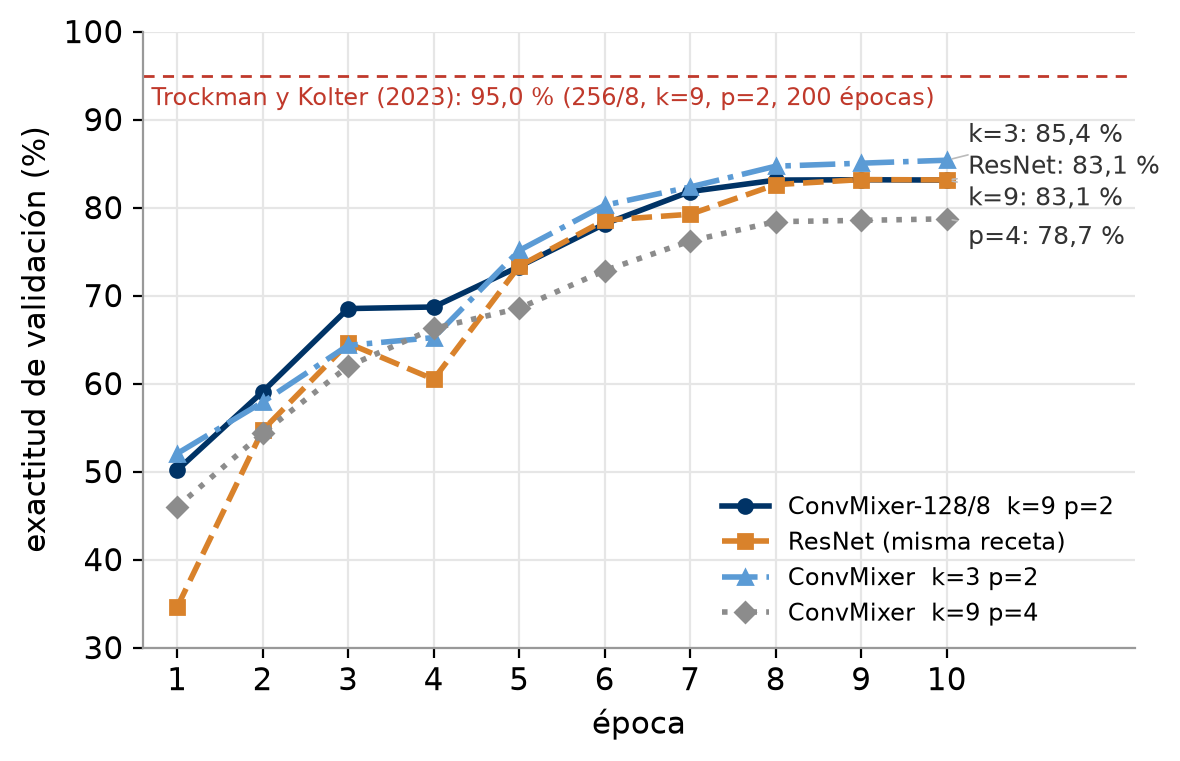
\includegraphics[width=0.49\textwidth]{f_curvas_validacion.png}\hfill
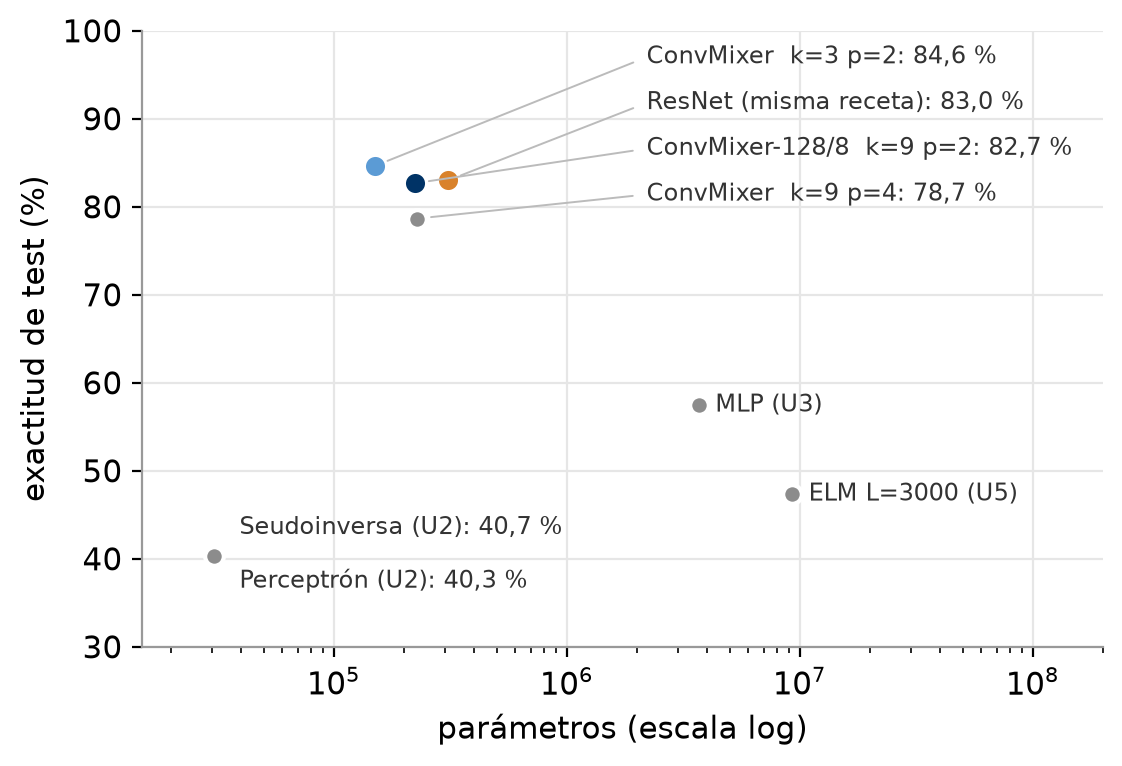
\includegraphics[width=0.49\textwidth]{f_comparacion.png}
\nota{Izquierda: exactitud en las 5\,000 imágenes de validación por época; la línea roja es el valor publicado para ConvMixer-256/8 con 200 épocas. Derecha: exactitud de test frente al número de parámetros (escala logarítmica). Elaboración propia a partir de \texttt{results/*.json}.}
\end{figure}

% Discusión de la réplica (se incluye en el informe). Los números salen de resultados.tex.
\subsection{Comparación con el artículo y causas de las diferencias}

\textbf{Valor absoluto.} El ConvMixer-128/8 llegó a \pct{\accCMnueve} en test, frente a \pct{95,0} que informa
el artículo para la misma configuración de núcleo y parche ($k=9$, $p=2$) con ancho 256. La diferencia de unos
12 puntos tiene causas concretas:
\begin{enumerate}
  \item \emph{Entrenamiento 20 veces más corto} (\epocasCNN{} épocas frente a 200). La Figura~\ref{fig:curvas}
  muestra que la validación se estabiliza en las últimas épocas sólo porque la tasa de aprendizaje llega a cero,
  no porque el modelo haya terminado de aprender.
  \item \emph{Modelo 3 veces más chico} (223\,k frente a 709\,k parámetros). En la Tabla~4 del artículo, pasar de
  $h=256$ a $h=128$ cuesta entre 1 y 2 puntos aun con 200 épocas.
  \item \emph{Sin RandAugment, mixup ni CutMix.} Según la Tabla~3 del artículo, quitar sólo RandAugment cuesta
  3 puntos.
  \item \emph{Protocolo más estricto}: el test se miró una sola vez y los hiperparámetros no se ajustaron sobre él.
\end{enumerate}

Para comprobar que la brecha se debe al cómputo y no a un error de implementación, entrené además el modelo en una
GPU gratuita de Google Colab (Tesla T4) con la receta del repositorio oficial de los autores para CIFAR-10
(\url{https://github.com/locuslab/convmixer-cifar10}): ConvMixer-256/8 con $k=5$ y $p=2$, RandAugment, ColorJitter,
\emph{random erasing} y 100 épocas, a unos \segColab{} segundos por época. Esa corrida llegó a \pct{\accColab} en test
\colabNota{} (Figura~\ref{fig:colab}). El artículo informa \pct{95,21} para esa configuración con 200 épocas. Es decir: con la receta
completa la implementación queda a menos de un punto del valor publicado, y la diferencia de la réplica en CPU se
explica por la escala del experimento.

\begin{figure}[h]
\caption{Réplica en GPU con la receta oficial de los autores (Google Colab, Tesla T4)}
\label{fig:colab}
\centering
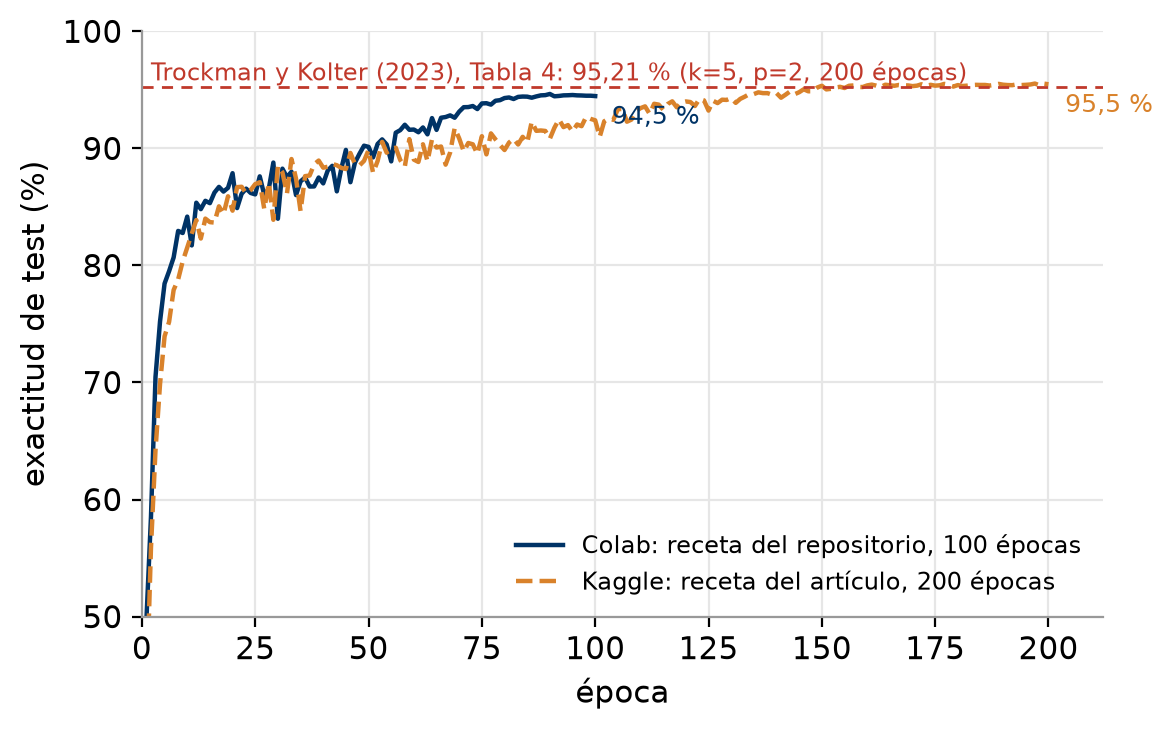
\includegraphics[width=0.62\textwidth]{f_colab.png}
\nota{Exactitud de test por época de ConvMixer-256/8 ($k=5$, $p=2$), sólo para seguimiento: el valor que se informa es el de la última época, sin elegir la mejor. La línea roja es el valor del artículo para la misma configuración con 200 épocas. Elaboración propia con el script \texttt{src/colab\_receta\_paper.py}.}
\end{figure}

\begin{table}[h]\small
\caption{La misma metodología con distinto cómputo: CPU propia, GPU de Colab, GPU de Kaggle y artículo}
\label{tab:cpugpu}
\centering
\resizebox{\textwidth}{!}{\begin{tabular}{lcccc}
\toprule
 & CPU propia (8 núcleos) & Google Colab (T4) & Kaggle (T4) & Artículo (GPU)\\
\midrule
Modelo & 128/8, $k=9$, $p=2$ & 256/8, $k=5$, $p=2$ & 256/8, $k=5$, $p=2$ & 256/8, $k=9$ o $5$, $p=2$\\
Parámetros & 223\,370 & 594\,186 & 594\,186 & 709\,k / 594\,k\\
Aumentación & escalado, recorte y espejo & + RandAugment, ColorJitter, borrado & Colab + mixup y CutMix & \texttt{timm} + mixup y CutMix\\
Weight decay & 0,01 & 0,005 & 0 & 0 (Tabla 4)\\
Épocas & \epocasCNN & \epColab & \epKaggle & 200\\
Tiempo por época & \minEpCPU{} min & \segColab{} s & \segKaggle{} s & no informado\\
Tiempo total & \minCMnueve{} min & \minColab{} min & \minKaggle{} min & no informado\\
Exactitud de test & \pct{\accCMnueve} & \pct{\accColab} & \pct{\accKaggle} & \pct{95,0} / \pct{95,21}\\
\bottomrule
\end{tabular}}
\nota{Una corrida por configuración, sin repetir semillas. Colab y Kaggle: se informa la última época, sin elegir la mejor; ambas con una GPU Tesla T4 (en Kaggle la sesión tenía dos, pero el script usa una). Colab entrenó \colabNota. Valores del artículo: Trockman y Kolter (2023, Tabla 4). Antes de la corrida de Colab que se informa hubo otra idéntica que se cortó en la época 84 (94,50 \%); el registro está en \texttt{results/}.}
\end{table}

La Tabla~\ref{tab:cpugpu} resume la comparación que me parece más interesante para discutir. Hay tres lecturas.
Primero, en un tiempo de reloj parecido (entre 1,5 y 2 horas), la GPU entrenó un modelo 2,7 veces más grande, con
muchas más épocas y con la aumentación completa, y ganó unos 12 puntos con el mismo código. Esto relativiza las
comparaciones entre arquitecturas: una parte de lo que se atribuye a ``un modelo mejor'' corresponde a ``un modelo que
recibió más cómputo y una receta más trabajada''. Es justamente la crítica que se le puede hacer al artículo cuando
compara contra números de otros trabajos.

Segundo, la receta cuenta. Pasar de la receta del repositorio (100 épocas, \pct{\accColab}) a la del artículo (200
épocas, mixup, CutMix y sin \emph{weight decay}) subió la exactitud de \pct{\accColab} a \pct{\accKaggle}, es decir, un
punto, y quedó 0,27 puntos por encima del \pct{95,21} publicado. Con una sola semilla por configuración, esa
diferencia con el artículo está dentro de lo que cabe esperar por azar (del orden de 0,2 a 0,3 puntos), así que lo
prudente es decir que la réplica \emph{iguala} el resultado publicado y no que lo supera. Tampoco puedo separar
cuánto aportó cada cambio (las épocas, mixup y CutMix, o el \emph{weight decay}), porque cambié todo junto; sólo el
artículo muestra que quitar mixup y CutMix casi no cambia el resultado (Tabla 3), lo que sugiere que el grueso viene de
las épocas.

Tercero, el costo. Con la misma GPU, la corrida de Kaggle tardó unos \minKaggle{} minutos (\segKaggle{} s por época)
y la de Colab unos \minColab{} minutos con la mitad de las épocas (\segColab{} s por época): en Kaggle cada época
fue más del doble de rápida. No sé a qué atribuirlo con certeza: la GPU es la misma (Tesla T4), pero cambió la
cantidad de procesos que cargan y aumentan las imágenes (4 en Kaggle y 2 en Colab) y, con RandAugment, esa parte corre
en la CPU y puede ser el cuello de botella. En la práctica, Colab gratuito nos negó la GPU por límite de uso a la
mañana siguiente y había cortado una corrida en la época 84; Kaggle ofrece unas 30 horas semanales y permite dejar la
corrida en segundo plano sin tener la pestaña abierta, lo que la hizo más cómoda y confiable para un entrenamiento
largo.

\textbf{Ablaciones: qué se reprodujo y qué no.}
\begin{itemize}
  \item \emph{Tamaño de parche: se reprodujo.} Con $p=4$ la exactitud cae a \pct{\accCMpcuatro} ($-$\difPatch{}
  puntos frente a $p=2$; en el artículo, $-2{,}4$). Con parches más grandes la resolución interna baja de
  $16\times16$ a $8\times8$ y el modelo pierde detalle, aunque corre unas 3,7 veces más rápido.
  \item \emph{Tamaño de núcleo: no se reprodujo.} Con $k=3$ obtuve \pct{\accCMtres}, es decir,
  \textbf{\difKernelAbs{} puntos a favor del núcleo chico}, al revés que en el artículo ($+2{,}3$ a favor de $k=9$
  con 200 épocas). Mi interpretación es que, con sólo \epocasCNN{} épocas, el modelo con menos parámetros y un sesgo
  local más fuerte converge antes, mientras que los núcleos grandes necesitan más entrenamiento para aprovechar el
  campo receptivo amplio. Los propios autores admiten esta posibilidad (``\emph{It could be that with more training
  iterations or more regularization, the effect of larger kernels would be more pronounced}'', Apéndice~B). Con una
  sola semilla por modelo, una diferencia de 2 puntos es indicativa pero no concluyente.
  \item \emph{ConvMixer frente a ResNet: empate.} La ResNet entrenada con la misma receta obtuvo \pct{\accResNet}
  frente a \pct{\accCMnueve} del ConvMixer ($k=9$), una diferencia de 0,3 puntos, menor que la variabilidad
  esperable entre semillas. El artículo encuentra una ventaja clara del ConvMixer en ImageNet, con modelos 100
  veces más grandes y 150 épocas. En esta escala no la observo.
  \item \emph{Velocidad: se reprodujo.} En inferencia, la ResNet procesa \tputResNet{} imágenes por segundo y el
  ConvMixer con $k=9$ y $p=2$, \tputCMnueve: la ResNet es \ratioTput{} veces más rápida, en línea con las Tablas~1
  y~2 del artículo. El entrenamiento muestra lo mismo: 110 minutos el ConvMixer y 32 minutos la ResNet.
\end{itemize}

\begin{figure}[h]
\caption{Ablaciones de la réplica frente a la Tabla 4 del artículo, y velocidad frente a exactitud}
\label{fig:ablaciones}
\centering
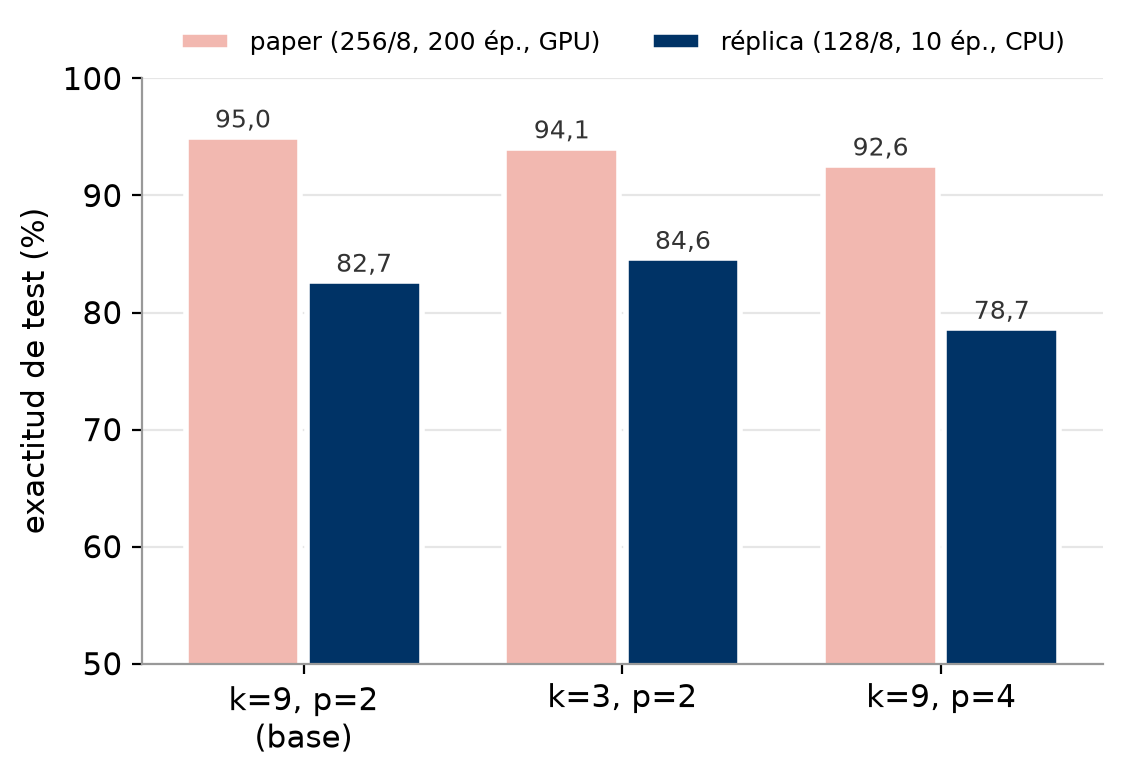
\includegraphics[width=0.49\textwidth]{f_ablaciones.png}\hfill
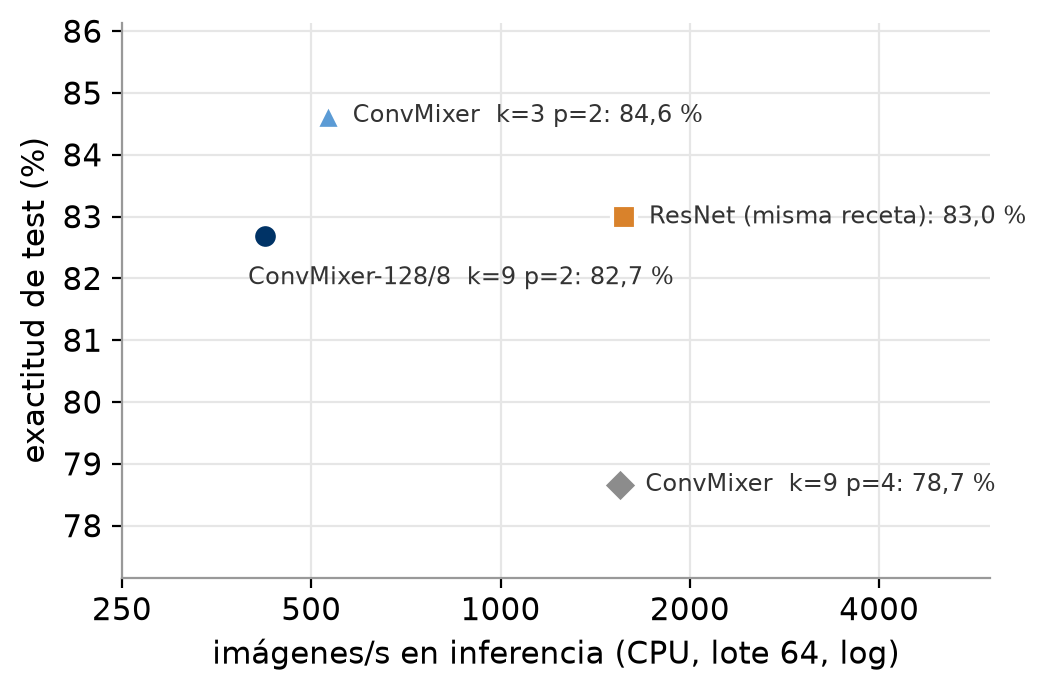
\includegraphics[width=0.49\textwidth]{f_throughput.png}
\nota{Izquierda: exactitud de test de la réplica (ConvMixer-128/8, 10 épocas, CPU) y del artículo (ConvMixer-256/8,
200 épocas, GPU; Trockman y Kolter, 2023, Tabla~4). Derecha: imágenes por segundo en inferencia, medidas en la misma
CPU con lotes de 64 (eje logarítmico). Elaboración propia.}
\end{figure}

\textbf{Los modelos del programa.} El orden de exactitud reproduce el recorrido del curso: perceptrón
(\pct{\accPerceptron}) $\approx$ seudoinversa (\pct{\accLineal}) $<$ ELM (\pct{\accELM}) $<$ MLP
(\pct{\accMLP}) $\ll$ CNN (\pct{\accResNet}--\pct{\accCMtres}). Los dos modelos lineales empatan porque comparten
la misma limitación: una frontera lineal sobre los 3\,072 píxeles. La validación cruzada eligió una regularización
fuerte ($\lambda=\lamCV$), señal de que el sistema está mal condicionado (píxeles vecinos casi colineales). La ELM
mejora al agregar no linealidad, pero sus rasgos aleatorios no aprovechan la estructura espacial; además, con
$N=45\,000\gg L=3\,000$ casi no sobreajusta, y su exactitud seguía subiendo con $L$, de modo que el límite fue la
memoria y no el método. El ML-ELM (\pct{\accMLELM}) quedó por debajo de la ELM simple: sus autoencoders comprimen
los píxeles a 1\,000 dimensiones con una reconstrucción lineal y pierden información útil para clasificar. El MLP,
con 16 veces más parámetros que el ConvMixer, queda 25 puntos abajo y sobreajusta (76\,\% en entrenamiento frente a
58\,\% en validación). Es la mejor ilustración del \emph{sesgo inductivo}: la localidad y los pesos compartidos de
la convolución valen más que los parámetros.

\begin{figure}[h]
\caption{Exactitud de test de todos los modelos de la réplica en CIFAR-10}
\label{fig:barras}
\centering
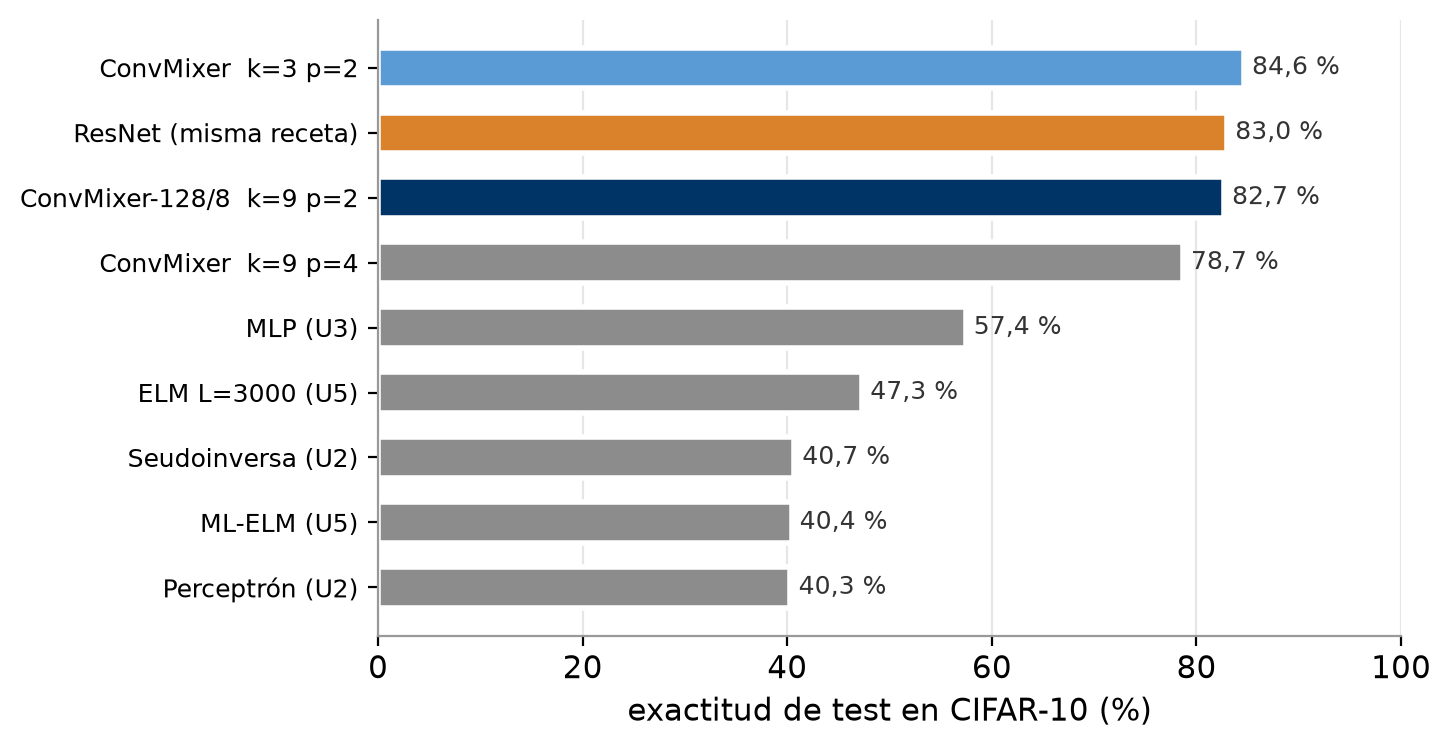
\includegraphics[width=0.75\textwidth]{f_barras.png}
\nota{Azul oscuro: modelo del artículo; naranja: línea de base ResNet; gris: ablaciones y modelos de las unidades 2,
3 y 5. Promedio de 3 semillas en los modelos no convolucionales. Elaboración propia.}
\end{figure}

\textbf{Limitaciones de esta réplica.} Una sola semilla por CNN, por costo de cómputo; 10 épocas; ningún
ajuste de hiperparámetros para la ResNet, igual que en el artículo; y modelos clásicos sobre píxeles crudos, sin
extracción de rasgos. Las diferencias menores a un punto no deben interpretarse.


% =================================================================
\section{Implicancias y reflexión crítica}
\textbf{¿Por qué este artículo?} Por tres razones. Primero, forma parte de la bibliografía que trabajé en la
materia \emph{Sistemas de Inteligencia Artificial} del ITBA (clase de Transformers y ViT), y analizarlo con la
lente de la Unidad~4 permite unir ambos cursos. Segundo, tiene una pregunta científica clara que admite una réplica
honesta en hardware modesto, porque el modelo cabe en seis líneas. Tercero, se vincula con mi tesis doctoral
(evaluación de la inestabilidad espinal con IA sobre tomografías y radiografías), donde la elección entre CNN,
transformers y modelos híbridos es una decisión de diseño concreta y los conjuntos de datos son chicos.

\textbf{¿En qué otros dominios podría usarse?} En \emph{segmentación de imágenes médicas}, porque la resolución
interna constante evita la pérdida de detalle del submuestreo y los núcleos grandes capturan contexto anatómico
amplio (por ejemplo, para la segmentación vertebral). También en microscopía y teledetección (imágenes grandes con
texturas repetitivas), en señales 1D como ECG o vibraciones (un ConvMixer 1D es inmediato) y en espectrogramas de
audio. Su eficiencia de datos lo hace atractivo cuando no hay millones de ejemplos.

\textbf{Conocimientos previos necesarios.} Convolución 2D y campo receptivo, convoluciones depthwise y pointwise
(MobileNet), BatchNorm, conexiones residuales, GELU, AdamW y programas de tasa de aprendizaje, técnicas de
aumentación (RandAugment, mixup, CutMix) y, para entender la motivación, el mecanismo de autoatención y el ViT.
De este curso fueron necesarias las unidades 3 (retropropagación y optimización) y 4 (convolución, SGD y
arquitecturas); la Unidad~1 fue clave para criticar la metodología (validación y test).

\textbf{Implicancias éticas.}
\begin{itemize}
  \item \emph{Costo ambiental y desigualdad de acceso}: 90 días-GPU para un punto de exactitud en ImageNet. Esta
  réplica muestra el otro lado: sin GPU sólo se puede verificar una versión reducida, y la investigación queda
  concentrada en quien tiene cómputo. Los autores lo reconocen (``\emph{limited compute}'').
  \item \emph{Reproducibilidad}: publicar el código y una implementación mínima es una buena práctica. Informar una
  sola corrida sin incertidumbre y ajustar mirando el test va en sentido contrario.
  \item \emph{Sesgos de los datos}: ImageNet tiene sesgos geográficos y culturales documentados, y un modelo
  ``mejor'' en ImageNet no es necesariamente mejor para otra población. En aplicaciones médicas eso exige validar
  externamente en datos locales.
  \item \emph{Doble uso}: los clasificadores de imágenes eficientes sirven tanto para diagnóstico como para
  vigilancia masiva.
\end{itemize}

\textbf{Ventajas y limitaciones frente a otros algoritmos.} La réplica ordena con claridad los algoritmos del
programa. Los modelos lineales (U2) no superan el \pct{\accLineal} porque una frontera lineal sobre píxeles no
captura la estructura de las clases. La ELM (U5) mejora con más neuronas aleatorias y se entrena en minutos sin
gradiente, pero sus rasgos aleatorios no aprovechan la geometría de la imagen. El MLP (U3) tiene 16 veces más
parámetros que el ConvMixer y queda muy por debajo. Las CNN (U4) dominan porque incorporan localidad y pesos
compartidos. Entre ellas, el ConvMixer logra la misma exactitud que la ResNet con menos parámetros, pero es bastante
más lento; esa parte de la conclusión del artículo se mantiene en mi réplica, no así su ventaja en exactitud.

% =================================================================
\section*{Uso de asistentes de IA}
Usé un asistente de IA (Claude Code) como apoyo para la programación y la revisión de la redacción. La
verificación de los resultados fue mía: comparé el conteo de parámetros con la ec.~(4), evalué el test una sola vez,
generé todos los números citados desde \texttt{results/*.json} con \texttt{src/figuras.py} y contrasté las
afirmaciones sobre el artículo con su texto.

\renewcommand{\refname}{Referencias}
\begin{thebibliography}{99}\small
\setlength{\itemindent}{-1.5em}\setlength{\leftmargin}{1.5em}\setlength{\itemsep}{2pt}
\bibitem[Ding et~al.(2022)]{replknet} Ding, X., Zhang, X., Han, J. y Ding, G. (2022). Scaling up your kernels to 31x31: Revisiting large kernel design in CNNs. En \emph{Proceedings of the IEEE/CVF Conference on Computer Vision and Pattern Recognition} (pp. 11963--11975). \url{https://doi.org/10.48550/arXiv.2203.06717}
\bibitem[Dosovitskiy et~al.(2021)]{vit} Dosovitskiy, A., Beyer, L., Kolesnikov, A., Weissenborn, D., Zhai, X., Unterthiner, T., Dehghani, M., Minderer, M., Heigold, G., Gelly, S., Uszkoreit, J. y Houlsby, N. (2021). An image is worth 16x16 words: Transformers for image recognition at scale. En \emph{International Conference on Learning Representations}. \url{https://doi.org/10.48550/arXiv.2010.11929}
\bibitem[Freund y Schapire(1999)]{freund} Freund, Y. y Schapire, R. E. (1999). Large margin classification using the perceptron algorithm. \emph{Machine Learning, 37}(3), 277--296.
\bibitem[He et~al.(2016)]{resnet} He, K., Zhang, X., Ren, S. y Sun, J. (2016). Deep residual learning for image recognition. En \emph{Proceedings of the IEEE Conference on Computer Vision and Pattern Recognition} (pp. 770--778). \url{https://doi.org/10.1109/CVPR.2016.90}
\bibitem[Huang et~al.(2012)]{elmreg} Huang, G.-B., Zhou, H., Ding, X. y Zhang, R. (2012). Extreme learning machine for regression and multiclass classification. \emph{IEEE Transactions on Systems, Man, and Cybernetics, Part B, 42}(2), 513--529.
\bibitem[Huang et~al.(2006)]{elm} Huang, G.-B., Zhu, Q.-Y. y Siew, C.-K. (2006). Extreme learning machine: Theory and applications. \emph{Neurocomputing, 70}(1--3), 489--501. \url{https://doi.org/10.1016/j.neucom.2005.12.126}
\bibitem[Kasun et~al.(2013)]{mlelm} Kasun, L. L. C., Zhou, H., Huang, G.-B. y Vong, C. M. (2013). Representational learning with ELMs for big data. \emph{IEEE Intelligent Systems, 28}(6), 31--34.
\bibitem[Krizhevsky(2009)]{cifar} Krizhevsky, A. (2009). \emph{Learning multiple layers of features from tiny images} [Informe técnico]. University of Toronto. \url{https://www.cs.toronto.edu/~kriz/cifar-10.html}
\bibitem[Liu et~al.(2021)]{swin} Liu, Z., Lin, Y., Cao, Y., Hu, H., Wei, Y., Zhang, Z., Lin, S. y Guo, B. (2021). Swin Transformer: Hierarchical vision transformer using shifted windows. En \emph{Proceedings of the IEEE/CVF International Conference on Computer Vision} (pp. 10012--10022). \url{https://doi.org/10.48550/arXiv.2103.14030}
\bibitem[Liu et~al.(2022)]{convnext} Liu, Z., Mao, H., Wu, C.-Y., Feichtenhofer, C., Darrell, T. y Xie, S. (2022). A ConvNet for the 2020s. En \emph{Proceedings of the IEEE/CVF Conference on Computer Vision and Pattern Recognition} (pp. 11976--11986). \url{https://doi.org/10.48550/arXiv.2201.03545}
\bibitem[Loshchilov y Hutter(2019)]{adamw} Loshchilov, I. y Hutter, F. (2019). Decoupled weight decay regularization. En \emph{International Conference on Learning Representations}. \url{https://doi.org/10.48550/arXiv.1711.05101}
\bibitem[Sandler et~al.(2019)]{sandler} Sandler, M., Baccash, J., Zhmoginov, A. y Howard, A. (2019). Non-discriminative data or weak model? On the relative importance of data and model resolution. En \emph{Proceedings of the IEEE/CVF International Conference on Computer Vision Workshops}.
\bibitem[Tolstikhin et~al.(2021)]{mixer} Tolstikhin, I., Houlsby, N., Kolesnikov, A., Beyer, L., Zhai, X., Unterthiner, T., Yung, J., Steiner, A., Keysers, D., Uszkoreit, J., Lucic, M. y Dosovitskiy, A. (2021). MLP-Mixer: An all-MLP architecture for vision. \emph{Advances in Neural Information Processing Systems, 34}, 24261--24272. \url{https://doi.org/10.48550/arXiv.2105.01601}
\bibitem[Touvron, Bojanowski et~al.(2021)]{resmlp} Touvron, H., Bojanowski, P., Caron, M., Cord, M., El-Nouby, A., Grave, E., Joulin, A., Synnaeve, G., Verbeek, J. y Jégou, H. (2021). \emph{ResMLP: Feedforward networks for image classification with data-efficient training} [Preimpresión]. arXiv. \url{https://doi.org/10.48550/arXiv.2105.03404}
\bibitem[Touvron, Cord et~al.(2021)]{deit} Touvron, H., Cord, M., Douze, M., Massa, F., Sablayrolles, A. y Jégou, H. (2021). Training data-efficient image transformers \& distillation through attention. En \emph{Proceedings of the 38th International Conference on Machine Learning} (pp. 10347--10357). PMLR. \url{https://doi.org/10.48550/arXiv.2012.12877}
\bibitem[Trockman y Kolter(2023)]{convmixer} Trockman, A. y Kolter, J. Z. (2023). Patches are all you need? \emph{Transactions on Machine Learning Research}. \url{https://doi.org/10.48550/arXiv.2201.09792}
\end{thebibliography}

\end{document}
